\pagestyle{fancy}
\rhead{\bfseries OCR A-Level Computer Science}
\chead{\mdseries \thepage}
\lhead{\bfseries Jonathan Kasongo \mdseries — May 2025/26}
\lfoot{\sffamily Candidate number: N/A}
\rfoot{\sffamily Centre number: N/A}

\chapter{Development}
\label{chap:development}

% Provided evidence of each stage of the iterative
% development process for a coded solution
% relating this to the break down of the problem
% from the analysis stage and explaining what they
% did and justifying why.

% Well structured and modular, code annotated, DRY

% Validation evidence 

\section{Development overview and sub-tasks}

We apply the principle of decomposition to our development
plan by splitting up the development of the system into 
a number of smaller sub-tasks. Each sub-task relates to it's
relevant circled number in our problem breakdown (see section 
\ref{sec:breakdown}).\\ \vspace{0.2cm}

\begin{longtblr}[
  caption={Development sub-tasks.}
]{
  colspec={cX}, hlines, row{1}={lightestgray}
}
  \hline
  Number & Sub-task \\
  \hline
  \circled{4} & Document the backend code throughout\\
  \circled{1} & Design home page \\
  \circled{2} & Design help page \\
  \circled{3} & Design login page \\
  \ldots & \ldots \\
  \hline
\end{longtblr}
\vspace{0.2cm}

Finally note that all the code for this project is open source
and freely available for you to view on github:
\texttt{<GH URL HERE>}

\section{Iteration 1}

During this iteration I wanted to finish up designs for each 
of the pages that will appear on our website. This should 
clear up sub-task \circled{1} and \circled{3}.

\subsubsection{Home page}

\begin{figure}[H]
\centering

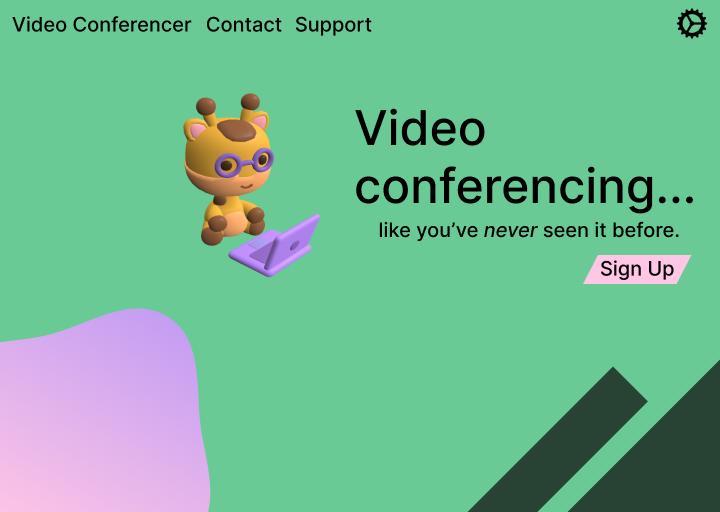
\includegraphics[scale=0.2]{Images/HomeUI_2.png}

\caption{2nd Mock up of the home page.}
\label{fig:ui2}
\end{figure}

\begin{figure}[H]
\centering

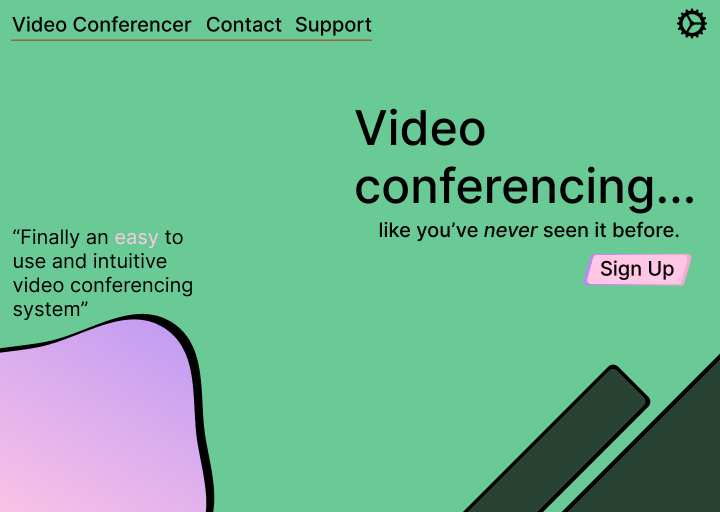
\includegraphics[scale=0.2]{Images/HomeUI_3.png}

\caption{3rd Mock up of the home page.}
\label{fig:ui3}
\end{figure}

I started by cleaning up the mock design for our home page.
The first mock up was a very basic outline for how I wanted to 
style the page, so in the next couple iterations I polished 
the design and added more designs to fill the web page. These
additions made the home page feel more complete and less 
bare-bones, consequently making the webpage feel more 
professional for the user. \\ \vspace{0.2cm}

The next step was to transfer this design into html and css. 
Since my designs made use of a collection of frequently used 
colours I concluded that it would be useful to be able to use
these colours as defined variables instead of having to write 
out their hex colour codes each time 
(see section \ref{sec:ui}). However the native CSS syntax 
looks something like this. (Taken from \url{https://www.w3schools.com/css/css3_variables.asp})

\begin{minted}[linenos, bgcolor=lightestgray]{css}
:root {
  --blue: #1e90ff;
  --white: #ffffff;
}
\end{minted}

I personally found this syntax particularly disgusting, 
after doing some research I came across this stack overflow 
answer \url{https://stackoverflow.com/a/1877358}. After digging
into exactly what "sass" and "less" were I decided to use sass
as an extension of my CSS because I liked the look of it's 
syntax better. Sass (\textbf{S}yntactically \textbf{A}wesome 
\textbf{S}tylesheet) is a CSS extension language that 
provides a new syntax for writing CSS as well as a number of 
features that prevent repetition in the code like variables, 
functions and more. The sass code is saved in a \texttt{.sass}
file then one can compile the sass code into CSS by using the
command \texttt{sass <sass file name> <output css file name>}.
\\ \vspace{0.2cm}

After blocking in the basic elements of our webpage the HTML 
and sass code looked like this.

\subsubsection{Prototype 1}

\underline{main.html}

\begin{minted}[linenos, bgcolor=lightestgray]{html}
<!DOCTYPE html>
<html>

<head>
  <meta charset="UTF-8">
  <meta name="viewport" content="width=device-width, initial-scale=1.0">
  <link href='https://fonts.googleapis.com/css?family=Inter' rel='stylesheet'>
  <link rel="stylesheet" href="styles.css">
  <title>Video-Conferencer</title>
</head>

<body>
  <div class="Headlines">

    <div class="Main_Headline">
      Video conferencing...
    </div>

    <div class="Sub_Headline">
      like you've never seen before.
    </div>

  </div>
</body>

</html>
\end{minted}

\underline{styles.sass}

\begin{minted}[linenos, bgcolor=lightestgray]{sass}
// Colour definitions
$Col_Main:       #69ca95
$Col_Secondary:  #284333
$Col_Tertiary:   #9a6442
$Col_Accent:     #ffc6e5
$Col_AccentDark: #c49df2

// Setting font and background colour
body
  background-color: $Col_Main
  font-family:      'Inter', sans-serif

// Styling for the main headline
.Main_Headline
  width:       701px
  height:      238px
  font-size:   96px
  font-weight: 600 
  position:    absolute
  top:         20%
  left:        43%

// Styling for the sub headline
.Sub_Headline
  width:       603px
  height:      101px
  font-weight: 500
  text-align:  center
  font-size:   40px
  position:    absolute
  top:         60%
  left:        46%
\end{minted}

This code produced our 1st prototype.

\begin{figure}[H]
\centering


\includegraphics[scale=0.2]{Images/Proto_home1.png}

\caption{Home page prototype 1}
\end{figure}

{\color{gray} \hrulefill} \vspace{0.2cm}

{\sffamily Client Feedback:} 
\begin{itemize}
  \item The headline and sub-headline are too far apart.
  \item The main headline takes up too much space on the page.
  \item The "never" isn't italicised.
\end{itemize}
{\color{gray} \hrulefill} 

\subsubsection{Prototype 2}

After writing the code for the first prototype I soon realised
that actually writing the text for the main headlines and 
manually positioning it would be a very tedious task. So I 
decided to instead export the headline as well as the graphic 
designs as \texttt{.svg} files from Figma. This means I
wouldn't have to worry about carefully positioning and spacing
the headlines individually and I could instead just position 
them as 1 vector image. The \texttt{.svg} image format was 
chosen because vector images never lose their resolution even
when scaled, you will still be able to see clean and crisp 
images no matter how much you zoom in, something which isn't
achievable with the \texttt{.jpg} or the \texttt{.png} formats.
In the rare case that \texttt{.svg} files are not supported
for the user's browser \footnote{Vector images are supported
by all browser except Internet Explorer 8 and below, and 
Android 2.3 browser and below.} we also provide fallback 
\texttt{.png} image files for these users. This ensures that 
users will be able to see the page's content no matter their 
choice of browser, hence improving the robustness of our
system.\\ \vspace{0.2cm}

Our code now looks like this.

\underline{main.html}
\begin{minted}[linenos, bgcolor=lightestgray]{html}
<!DOCTYPE html>
<html>

<head>
  <meta charset="UTF-8">
  <meta name="viewport" content="width=device-width, initial-scale=1.0">
  <link href='https://fonts.googleapis.com/css?family=Inter' rel='stylesheet'>
  <link rel="stylesheet" href="styles.css">
  <title>Video-Conferencer</title>
</head>

<body>

  <div id="Headline_container">
    <object id="Headline" data="Images/Headline_text.svg" type="image/svg+xml">
      <img src="Images/Headline_text.png">
    </object>

    <object id="Sign_up" data="Images/Sign_up.svg" type="image/svg+xml">
      <img src="Images/Sign_up.png">
    </object>
  </div>

  <div id="Bot_left_graphic_container">
    <object id="Bot_left_graphic" data="Images/Bot_left_graphic.svg" type="image/svg+xml">
      <img src="Images/Bot_left_graphic.png">
    </object>
  </div>

  <div id="Bot_right_graphic_container">
    <object id="Bot_right_graphic" data="Images/Bot_right_graphic.svg" type="image/svg+xml">
      <img src="Images/Bot_right_graphic.png">
    </object>
  </div>

</body>

</html>
\end{minted}

\underline{styles.sass}
\begin{minted}[linenos, bgcolor=lightestgray]{sass}
// Colour definitions
$Col_Main:       #69ca95
$Col_Secondary:  #284333
$Col_Tertiary:   #9a6442
$Col_Accent:     #ffc6e5
$Col_AccentDark: #c49df2

// Setting font and background colour
body
  height:           100vh
  margin:           0
  background-color: $Col_Main
  font-family:      'Inter', sans-serif
  overflow:         hidden

// Positioning the headline svg
#Headline_container
  position: relative
  top:      10%
  left:     45%

// Positioning the signup svg
#Sign_up
  position: absolute
  top:      75%
  left:     35%

// Positioning the bottom left graphic svg
#Bot_left_graphic_container
  position: relative
  top:      0%

// Positioning the bottom right graphic svg
#Bot_right_graphic_container
  position: relative
  left:     50%
  bottom:   75%
\end{minted}

This code produced our 2nd prototype.

\begin{figure}[H]
\centering

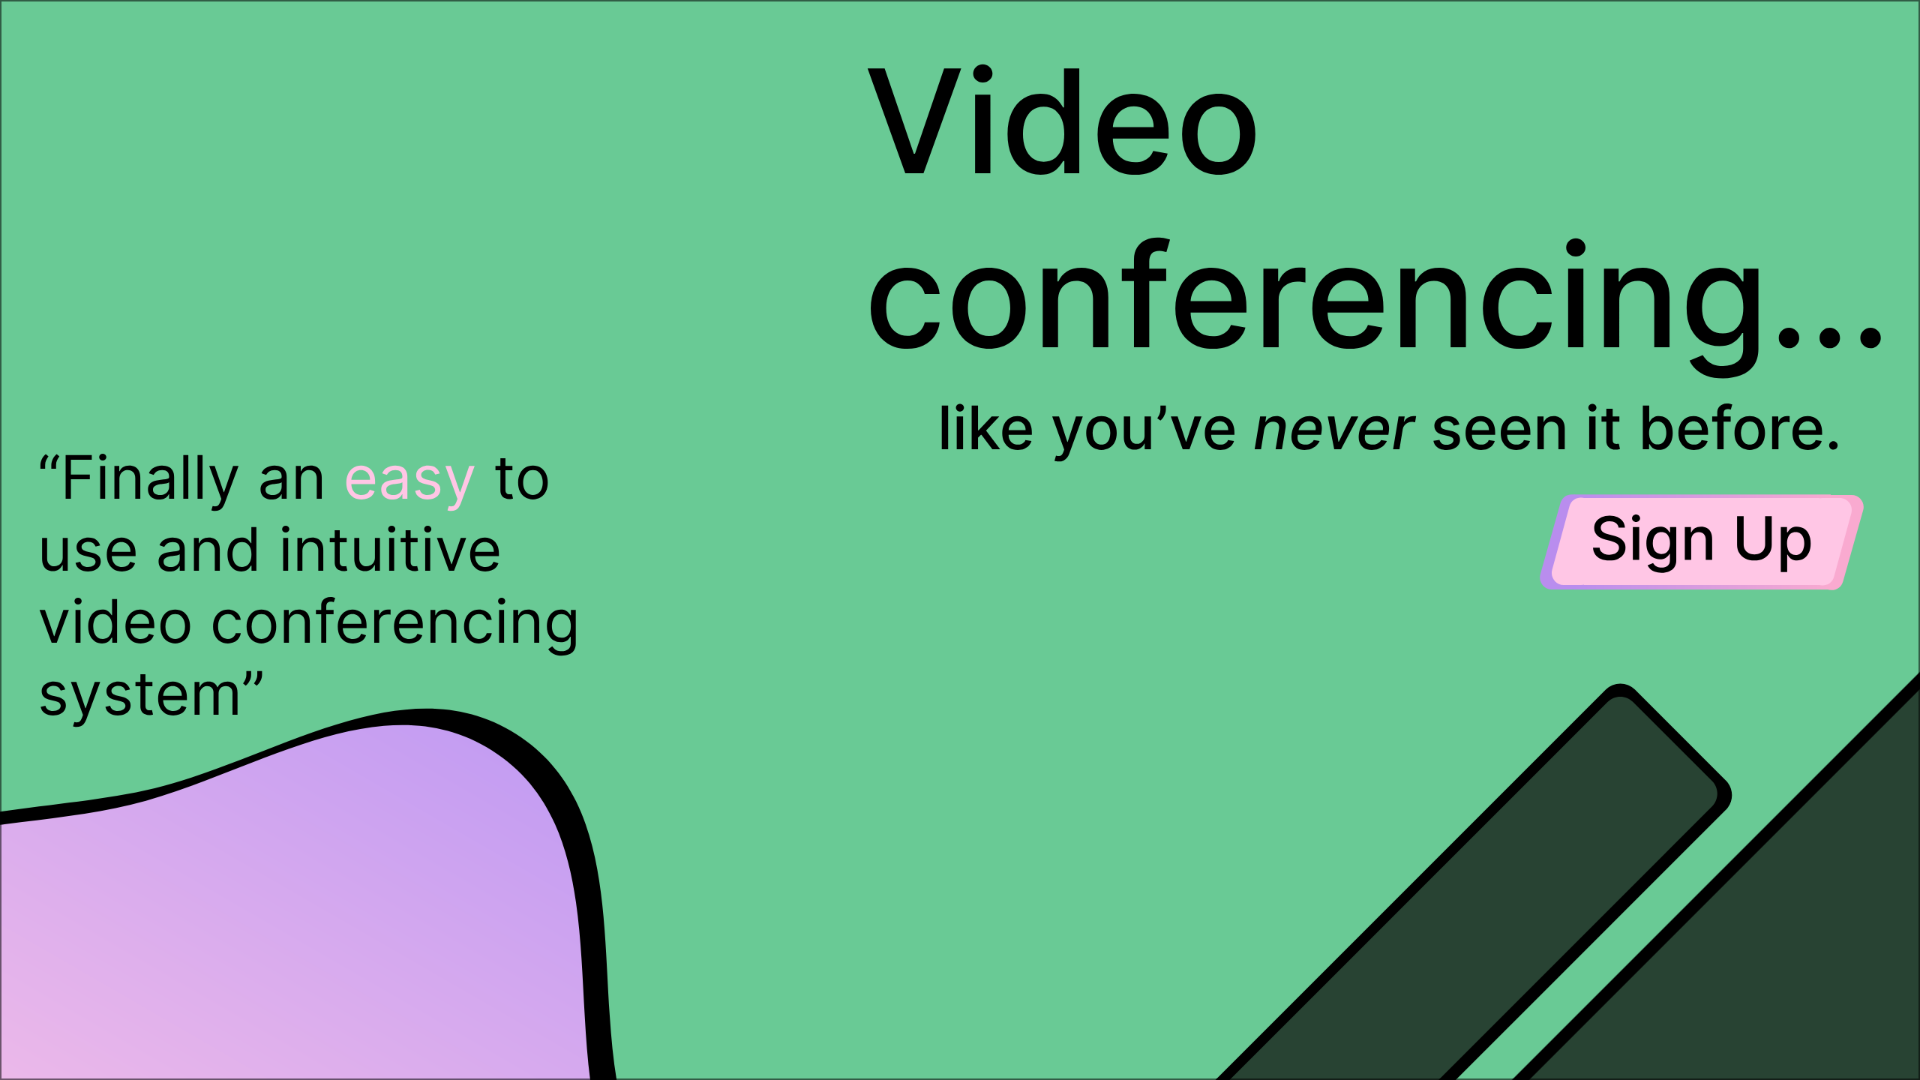
\includegraphics[scale=0.2]{Images/Proto_home2.png}

\caption{Home page prototype 2}
\end{figure}

{\color{gray} \hrulefill} \vspace{0.2cm}

{\sffamily Client feedback:}

\begin{itemize}
  \item We are still lacking a navigation bar at the top.
  \item All the elements feel as though they take up too much space on the page.
\end{itemize}

{\color{gray} \hrulefill} 

\subsubsection{Prototype 3}

After reviewing the design holistically, I felt that I could 
have done a better job designing the page to contribute to 
creating a professional looking system, so I re-did my 
designs in Figma. The graphic designs on our previous 
prototype designs were nice but they felt "too much",
so I decided I should tone back the designs and focus on 
simplicity. Similarly the choice for the background colour
was too bright and vibrant and didn't allow other elements 
to stand out as much as they should. In designing the revised 
prototype I took inspiration from the design of the 
Zen browser home-page \url{https://zen-browser.app/}. They 
simply have a navigation bar, a main and sub headline, a call
to action button and some testimonials along the bottom. Here
is the newest design. (Of course after making such significant
changes I contacted my client and asked for permission to
change to this new design and he agreed).

\begin{figure}[H]
\centering

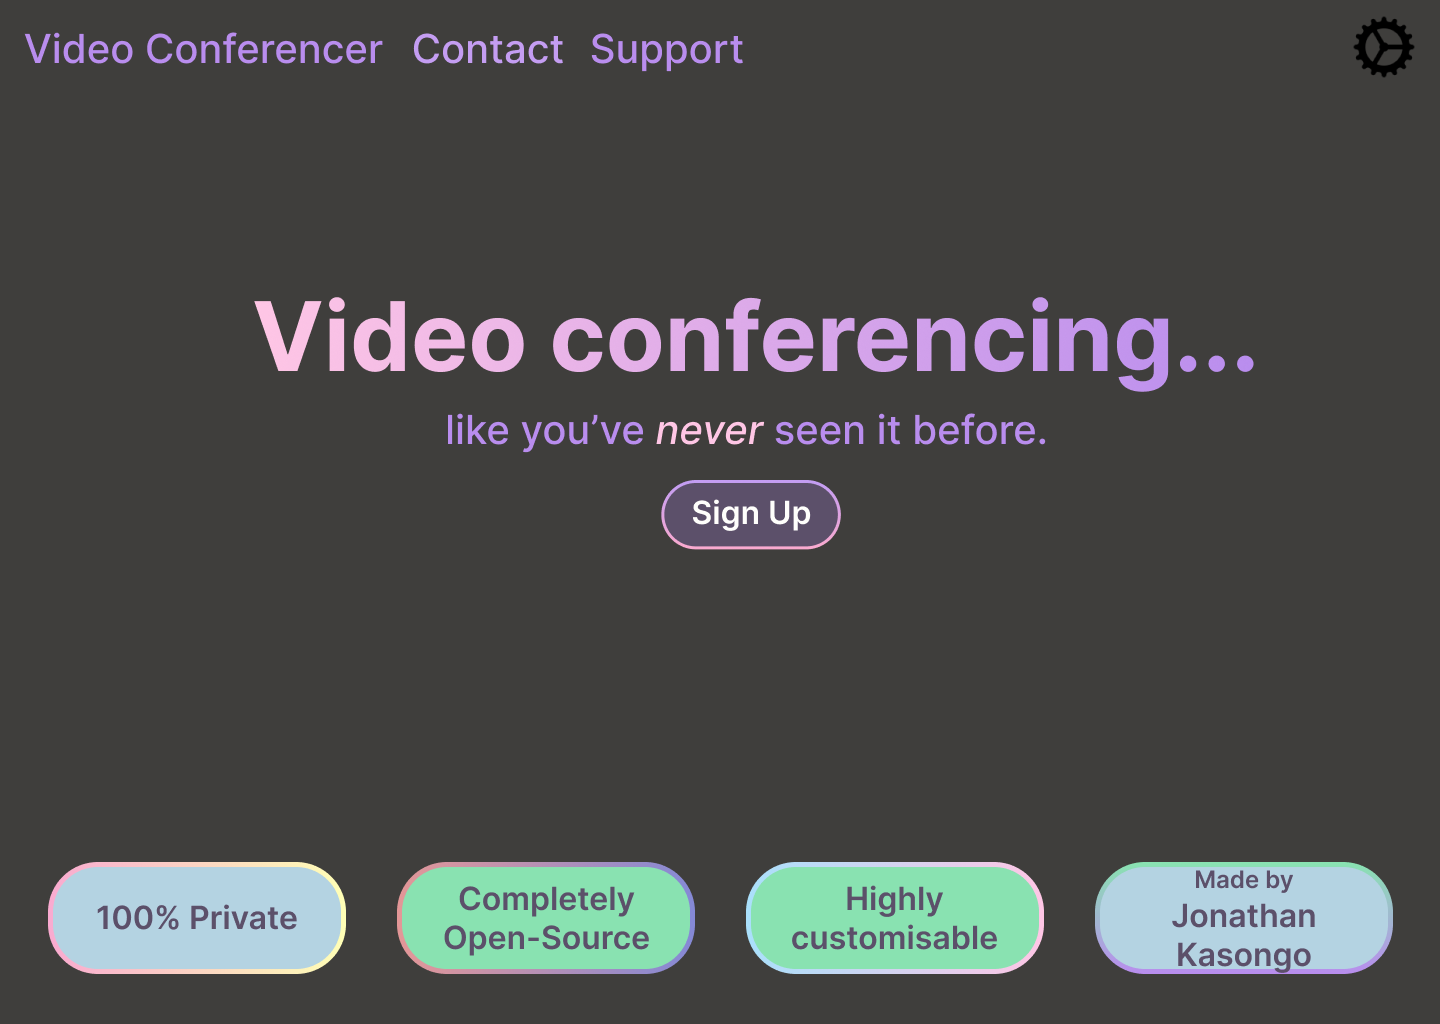
\includegraphics[scale=0.2]{Images/HomeUI_4.png}

\end{figure}

\subsubsection{Login page}
